\section{Anwendung in der Praxis}

\subsection{Implementierung von EDA im RAP Umfeld}
  Das Ziel dieses Abschnitts ist es, darzustellen wie die bisher dargelegten Konzepte in der Entwicklung eines Prototyps angewandt wurden und somit ein 'Proof of Concept' erstellt wurde. Hierzu soll zuerst der technische Prozess der Implementierung und schließlich der Aufbau des Prototyps dargestellt werden.\\

  \subsubsection*{Implementierung aufseiten der BTP}
    
  \begin{figure}[H]
    \centering
    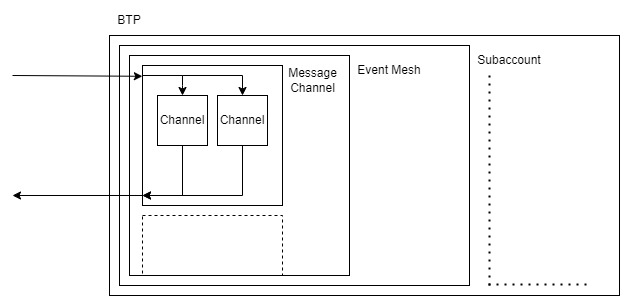
\includegraphics[width=0.8\textwidth]{event processing.jpg}
    \caption[BTP Event-Mesh]{Aufbau des BTP Event-Mesh \footnotemark}
    \label{EMprocessing}
  \end{figure}
  \footnotetext{Eigene Darstellung}
  Wie bereits im theoretischen Teil der Arbeit kurz angerissen und in Abbildung \ref{EMprocessing} dargestellt soll ein SAP-spezifischer Cloud-Dienst verwendet werden, der als Event-Platform fungieren soll. Die Konfiguration dieses Dienstes beginnt mit der Einrichtung eines Unteraccounts in einer \ac{BTP} Instanz. Dieser Unteraccount wird dann mit dem Event-Mesh Dienst verknüpft. Der Dienst kann hierbei über ein User Interface administriert werden. Hier kann dann ein sogenannter Message-Client erstellt werden. Es handelt sich hierbei um die aktive Komponente des Event Mesh, die Nachrichten senden und empfangen kann. Auf Ebene des Message-Clients können zudem Regeln konfiguriert werden, die Nachrichten und Ereignisse nach Themen und Absender filtern. Innerhalb des Message-Clients können dann sogenannte Queues erstellt werden. Diese Queues sind die eigentlichen Kommunikationskanäle, über die Nachrichten ausgetauscht werden. Queues horchen auf Ereignisse mit bestimmten Themen und halten diese so lange bis sie von einem Subscriber konsumiert werden. Zum Beispiel kann einmal durchgegangen werden, wie ein Ereignis, das durch die Änderung einer Reisebuchung ausgelöst wurde, von dem Event Mesh verarbeitet wird. Um ein Ereignis an ein Message-Channel zu senden, muss ein sogenanntes Service Binding generiert werden. Hierbei handelt es sich um ein Artefakt, 
   \begin{wrapfigure}{l}{7cm}
   \centering
   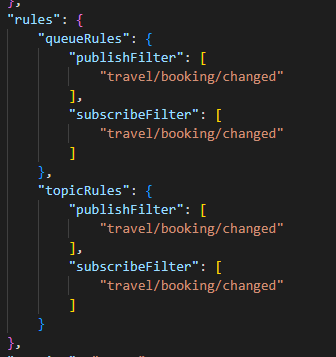
\includegraphics[width=0.4\textwidth]{messagechannelconfig.png}
   \caption[Message-Channel Konfiguration]{Regeln für die Konfiguration des Message-Channels \footnotemark}
   \label{MesChannelConfig}
 \end{wrapfigure}
 \footnotetext{Eigene Darstellung} 
  das in einem strukturierten Dateiformat sämtliche Verbindungs- und Authentifizierungsdaten enthält.  Der Publisher kann die Informationen aus diesem Dokument, die pro Message-Channel eindeutig sind, nutzen um eine Verbindung zum Event Mesh herzustellen. Der Publisher kann dann eine Nachricht an das Event Mesh senden. Diese Nachricht enthält neben dem eigentlichen Ereignis auch Metadaten, die das Ereignis beschreiben.  
  Hierzu gehören unter anderem das Thema des Ereignisses, der Absender und der Zeitpunkt der Erstellung. Im Kontext des Beispiels könnte das Thema des Ereignisses 'travel.booking.changed' sein, wobei das Thema aber frei wählbar ist. Um das Ereignis zu verarbeiten, müsste nun im Message Channel eine Queue konfiguriert sein, die auf dieses Thema horcht. Damit würde das Ereignis in der Queue landen und könnte von einem Subscriber konsumiert werden. 
  Aufseiten des Message-Channels müsste zudem eine Regel formuliert sein, die zulässt, dass Ereignisse mit dem Thema 'travel.booking.changed' angenommen werden. Die Formulierung dieser Regeln wird in der Erstellung des Channels im Rahmen einer Konfigurationsdatei, die service descriptor genannt wird, vorgenommen, wie in Abbildung \ref{MesChannelConfig} dargestellt und erlaubt auch die Verwendung von Wildcards. Eine Regel, die im Beispiel eine Annahme des Ereignisses erlauben würde, könnte 'travel/booking/*' oder 'travel/*' sein.\\

  Sind diese Schritte vorgenommen, ist das grundlegende Gerüst der Event-Plattform fertiggestellt. An das Event Mesh können Publisher und Subscriber auf verschiedene Weisen angebunden werden. Vorgeschrieben ist nur, dass die Ereignisse, die diese erzeugen und konsumieren dem in Abschnitt \ref{cloudev} beschriebenen Cloud Event Spezifikationen folgen und somit alle relevanten Metadaten enthalten.\\

  \subsubsection*{Implementierung aufseiten des SAP S/4 Systems}
  Das Grundgerüst einer Fiori Anwendung ist mithilfe der \ac{ADT} schnell erstellt. Auf Basis einer Tabelle als Datenquelle können alle Artefakte eines fertigen \ac{BO} generiert werden. Daraus ergibt sich eine vollständige transaktionale Anwendung, mit der Datensätze erstellt, gelesen, geändert und gelöscht werden können. An späterer Stelle wird noch einmal näher auf die Verwendung des \ac{BO} als Publisher eingegangen.\\
  \begin{figure}[H]
    \centering
    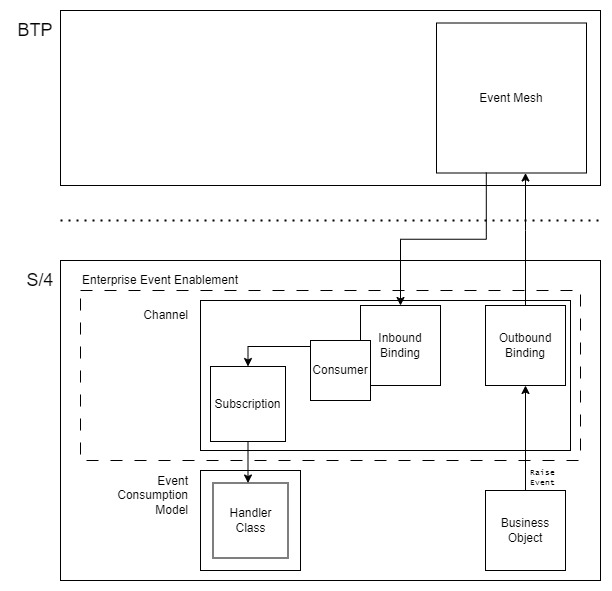
\includegraphics[width=0.8\textwidth]{eventingstructure.jpg}
    \caption[Eventing in SAP S/4]{Eventing in SAP S/4 unter Verwendung des BTP Event Mesh \footnotemark}
    \label{BEstructure}
  \end{figure}
  \footnotetext{Eigene Darstellung}
  \clarify{Lieber rechts nach links}

  Die Artefakte, die benötigt werden, um Ereignisse im S/4 System zu senden und zu empfangen sind in Abbildung \ref{BEstructure} dargestellt. Gekapselt werden sie in einem Paket, das Enterprise Event Enablement genannt wird. Für die Kommunikation mit dem Event Mesh in der Cloud muss als grundlegendes Artefakt ein Channel angelegt werden. Dieser kann automatisch generiert werden, indem der Service Key angegeben wird. Wie im vorherigen Abschnitt beschrieben, enthält dieser Service Key alle notwendigen Angaben über Endpunkte, Authentifizierung und Protokolle um sich mit dem Cloud-Service zu verbinden. Somit kann mit dem Channel diese Verbindung abgedeckt werden. Innerhalb des Channels können dann sogenannte Bindings angelegt werden. Ein Binding enthält die Konfiguration der Themen, die durch den Channel an das Event-Mesh weitergeben werden sollen. Unterschieden wird in Outbound- und Inbound-Binding. Tritt im System ein Ereignis auf, dass mit einem Thema im Outbound Binding übereinstimmt, kümmert sich der Channel darum, dieses an das Event Mesh weiterzugeben. Auf der anderen Seite ist das Inbound-Binding an sich auch nur eine Spezifikation von Themen, die der Channel vom Event Mesh empfangen kann. Die eigentliche Abholung der Ereignisse wird mit der sogenannten Subscription konfiguriert, die die Basis für das Erstellen eines hintergründig laufenden Jobs bildet, welcher dann die Ereignisse aus der Queue des Message-Clients abholt und an die richtigen stellen im S/4 System weiterleitet.\\

Soll nun also ein Ereignis durch ein \ac{BO} erzeugt werden, muss zuerst einmal in der Behavior Definition diese \ac{BO} definiert werden, dass es ein Ereignis senden kann. 

\begin{lstlisting}
  // dieses BO kann ein Ereignis mit dem Namen TravelCancelled senden, welches Nutzdaten vom Typ ZRU_CanceledReason enthaelt
  event TravelCancelled parameter ZRU_CanceledReason;
\end{lstlisting}

Wenn das getan ist, kann ein Artefakt, das Event-Binding, erstellt werden, das im \ac{BO} liegt und dazu dient, Ereignisse die Im \ac{BO} erzeugt werden, an den Event-Channel weiterzugeben.\\
Schlussendlich muss nur noch im Programmcode der Behavior-Implementation das Ereignis auch tatsälich ausgelößt werden. Hierzu wird die Methode RAISE ENTITY EVENT aufgerufen, die als Parameter den Namen des Ereignisses und optional die Nutzdaten des Ereignisses mit dem Schlüsselwort FROM VALUE erwartet.\\

\begin{lstlisting}[language=ABAP]
  " löst ein Ereignis mit einem Parameter aus
  RAISE ENTITY EVENT zru_r_traveltp~TravelCancelled
  FROM VALUE #( ( TravelID = 4 %param ='aTestEvent' ) ).
\end{lstlisting}

Wird dieser Programmcode ausgeführt, wird das Ereignis ausgelöst und mithilfe der bis jetzt besprochenen Artefakte an das Event Mesh weitergegeben.\\

Es bleibt zu beleuchten, wie ein Ereignis in S/4 konsumiert wird. Wenn Inbound-Binding sowie Subscription definiert sind, kann mithilfe der \ac{ADT} ein Event Consumption Model angelegt werden. Wie bereits in Abschnitt \ref{ecm} beleuchtet handelt es sich hierbei um eine Sammlung an Artefakten, deren relevanteste Aufgabe es ist, eine \ac{ABAP}-Klasse bereitzustellen, deren Methoden immer dann aufgerufen werden, wenn ein Ereignis konsumiert wurde. Zur Generation dieses Event Consumption Models wird eine strukturierte Beschreibung des Ereinisses benötigt, welches verarbeitet werden soll. Im SAP Kontext erfolt diese Beschreibung nach dem offenen Standart von AsyncAPI.\footnote{Auf diesen Standard soll an dieser Stelle nicht näher eingegangen werden, da das Artefakt, das ein Ereignis beschreibt in den allermeisten Fällen automatisch generiert werden kann.} Mithilfe dieser Ereignisbeschreibung kann dann ein Event Consumption Model generiert werden. Teil dieses Models ist eine Klasse, in der schlussendlich eine Methode implementiert werden kann, die immer dann aufgerufen wird, wenn ein Ereignis konsumiert wurde.\\

\subsection{Implementierung des Prototyps}
\subsubsection*{Anforderungen}
Der Prototyp soll aus einer Beispielanwendung bestehen, die auf Basis eines \ac{BO} eine Fiori UI Frontend Anwendung bereitstellt. Die Anwendung soll dabei die grundlegenden Funktionen eines \ac{BO} implementieren, also das Erstellen, Lesen, Ändern und Löschen von Datensätzen. Die Anwendung soll dabei auf einem SAP S/4 System laufen und die Daten in der HANA Datenbank des Systems speichern. Zudem soll in jeder Speichersequenz des \ac{BO}s ein Business Event ausgelöst werden. An anderer Stelle im System soll ein Subscriber auf das Ereignis reagieren und es sowohl in einer Log-Datenbank persistieren als auch eine Notification an einen Benutzer senden.
\subsubsection*{Der Prototyp}
Die inhaltliche Grundlage bildet nach SAP-Kovention eine Anwendung aus dem Bereich des Reisemanagements. Das \ac{BO} 'Travel' soll hierbei die Daten einer Reise speichern. Es können hierbei Datensätze erstellt, verändert und gelöscht werden. Relevant ist vor allem die Speicheraktion, denn hier wurde die zusätzliche Programmlogik implementiert, die das Ereignis generiert. Im Sinne des Proof of Concept wird ein Ereignis mit einem eigenen Datentyp als Nutzdaten verschickt, der einen Code und eine Beschreibung enthält. 
Empfangen wird das Ereignis durch ein Event Consumption Model, welches eine Benachrichtigung an einen Benutzer sendet und das Ereignis in einer Datenbank persistiert.\\
\subsubsection*{Nutzen und Weiterentwicklungsmöglicheiten}
Mit diesem Prototyp wurde vor allem gezeigt, wie es möglich ist, im gegeben Softwareumfeld eine \ac{EDA} zu implementieren. Zudem wurde eine Übersicht über die Schritte gewonnen, die nötig sind um das zu erreichen. 
Einen produktiven Nutzen hat das System nicht weiter, es ist aber denkbar, dass die Nutzung von Nutzerbenachrichtigungen, die über \ac{EDA} gesteuert werden weiter verfolgt wird.\\